\section{Разработка критериев оптимизации и анализ фронта Парето}\label{sec:ch4/sec6}
\subsection{Выбор и обоснование критериев качества управления}\label{sec:ch4/sec6/subsec1}

Разработка и выбор критериев качества управления является одним из основных этапов многокритериальной
оптимизации параметров пневмопривода, поскольку выбор критериев, являющихся противоречивыми
и взаимоисключающими, определяет возможные стратегииуправления и область допустимых решений.

В результате проведенного анализа литературы установлено, что основными направлениями
повышения производительности являются увеличение быстродействия и точности
позиционирования, при этом существенную роль играет надежность
привода. Дискретный характер управления пневмоприводом обуславливает частые
переключения распределителей, что приводит к ускоренной наработке ресурса и снижению надежности системы.

На основании выявленной специфики задачи предлагается использование следующих критериев качества:

Первый критерий характеризует точность позиционирования и качество переходного процесса:

\begin{equation}
	J_1 = \int_0^T \left(w_1\left(\frac{e(t)}{e_{max}}\right)^2 + w_2\left(\frac{\dot{e}(t)}{\dot{e}_{max}}\right)^2\right)dt
\end{equation}

Данный критерий представляет собой модифицированный интегральный квадратичный критерий.
Первое слагаемое оценивает точность позиционирования через квадрат нормированной ошибки,
второе -- учитывает динамику её изменения. Квадратичная форма обеспечивает
более жесткое штрафование больших отклонений. Нормирование на
максимальные значения $e_{max}$ и $\dot{e}_{max}$ обеспечивает
безразмерность и соизмеримость составляющих. Весовые коэффициенты
$w_1$ и $w_2$ позволяют регулировать соотношение между статической точностью и динамическими характеристиками.

Второй критерий оценивает ресурсную нагрузку на исполнительные механизмы:

\begin{equation}
	J_2 = \alpha \cdot f_{rms} + \beta \cdot \frac{N}{N_{max}}
\end{equation}
где $f_{rms}$ -- среднеквадратичная частота переключений:

\begin{equation}
	f_{rms} = \sqrt{\frac{1}{N}\sum_{i=1}^N f_i^2}
\end{equation}

Использование среднеквадратичного значения частоты позволяет
придать больший вес высокочастотным переключениям, наиболее
критичным для механического износа компонентов. Второе слагаемое
учитывает общее количество переключений относительно
допустимого значения. Коэффициенты $\alpha$ и $\beta$ определяют
баланс между динамической и статической составляющими износа.

Третий критерий оценивает быстродействие системы:
\begin{equation}
	J_4 = \gamma_1 t_s + \gamma_2 t_r + \gamma_3 \int_0^T t|e(t)|dt
\end{equation}

Критерий комбинирует основные временные характеристики:
время регулирования $t_s$, характеризующее длительность
переходного процесса, время нарастания $t_r$, отражающее
скорость начального отклика, и интегральный член,
учитывающий длительность существования ошибки с
нарастающим весом. Коэффициенты $\gamma_1$, $\gamma_2$ и $\gamma_3$ позволяют
настраивать значимость различных составляющих быстродействия.

Выбранные критерии обладают следующими ключевыми свойствами:

безразмерность и нормированность, обеспечивающие соизмеримость;
физическая интерпретируемость, позволяющая формулировать инженерные требования;
вычислительная эффективность при численной оптимизации;
комплексность оценки различных аспектов функционирования системы.

Данные критерии являются противоречивыми, поскольку улучшение
одного показателя, как правило, влечет ухудшение других.
В частности, повышение быстродействия обычно требует более интенсивного
управления и, следовательно, увеличивает
число и частоту переключений. Улучшение
точности позиционирования может потребовать дополнительных
корректирующих воздействий, что отражается на всех остальных критериях.


\subsection{Визуализация и анализ фронта Парето}\label{sec:ch4/sec6/subsec2}

Визуализация и анализ фронта Парето представляет собой важный этап многокритериальной оптимизации,
позволяющий исследовать полученные решения и выявить характерные особенности пространства
поиска. Методы визуализации существенно различаются в зависимости от размерности пространства целевых функций.

Для случая двух критериев оптимизации естественным способом визуализации является представление
решений в декартовой системе координат, где по осям откладываются значения целевых функций. В этом
случае фронт Парето отображается в виде кривой, позволяющей наглядно оценить компромисс между
критериями. График фронта парето представлен на рисунке \ref{img4:pareto_front_2_example}.

\begin{figure}[ht]
	\centerfloat{
		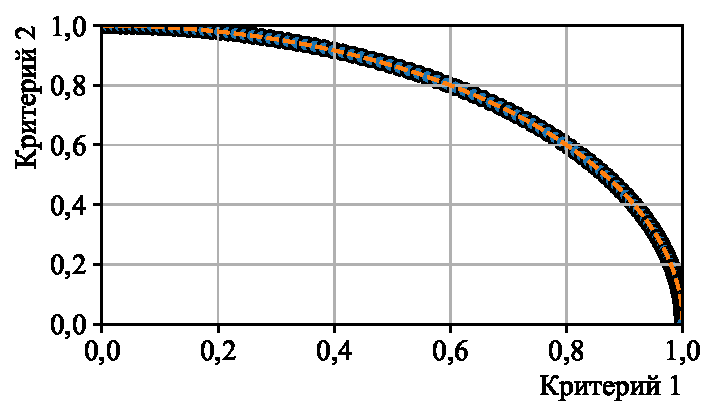
\includegraphics[]{part4/pareto_front_2_example.pdf}
	}
	\caption{Пример графика фронта Парето для двух критериев}
	\label{img4:pareto_front_2_example}
\end{figure}

Математически данное отображение описывается как:
\begin{equation}
	P = {(f_1(\mathbf{x}), f_2(\mathbf{x})) | \mathbf{x} \in \Omega },
\end{equation}
где $f_1(\mathbf{x})$ и $f_2(\mathbf{x})$ -- значения целевых функций, $\Omega$ -- допустимое множество решений.


При наличии трех целевых функций теоретически возможно применение трехмерной визуализации, где фронт Парето представляется поверхностью в пространстве критериев:
\begin{equation}
	P = {(f_1(\mathbf{x}), f_2(\mathbf{x}), f_3(\mathbf{x})) | \mathbf{x} \in \Omega }.
\end{equation}

График фронта парето для трех критериев представлен на рисунке \ref{img4:pareto_front_3_example} 

\begin{figure}[ht]
	\centerfloat{
		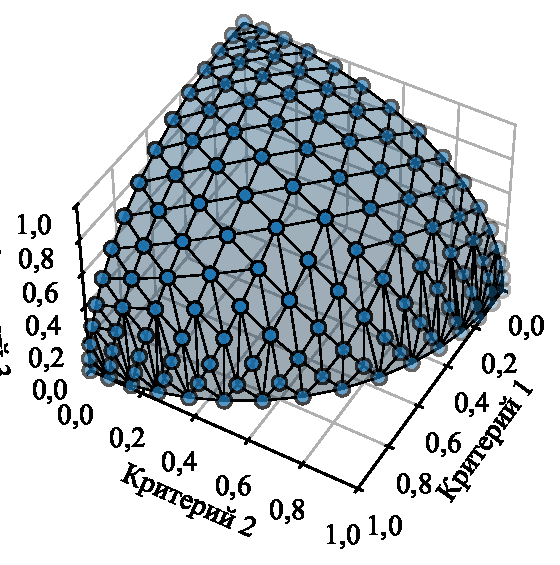
\includegraphics[]{part4/pareto_front_3_example.pdf}
	}
	\caption{Пример графика фронта Парето для трех критериев}
	\label{img4:pareto_front_3_example}
\end{figure}

Однако трехмерная визуализация зачастую оказывается малоинформативной в силу ряда существенных ограничений:

\begin{enumerate}
	\item сложность восприятия пространственных отношений на плоском экране или бумаге;
	\item эффект перекрытия точек и участков поверхности при проекции;
	\item затруднённость количественной оценки взаимного расположения решений;
	\item ограниченные возможности интерактивного взаимодействия при анализе статических изображений.
\end{enumerate}

При числе критериев более трех, а также для повышения информативности визуализации
в трехмерном случае, целесообразно применение специальных методов отображения на плоскость.
Одним из эффективных подходов является angular mapping, позволяющий отобразить точки
многомерного пространства на плоскость с сохранением угловых соотношений между векторами решений.

В рамках метода angular mapping каждое решение $\mathbf{x}$ характеризуется вектором значений целевых функций:
\begin{equation}
	\mathbf{f}(\mathbf{x}) = (f_1(\mathbf{x}), f_2(\mathbf{x}), ..., f_m(\mathbf{x}))
\end{equation}

Отображение на плоскость осуществляется путем вычисления полярных координат $(\rho, \theta)$:
\begin{equation}
	\begin{cases}
		\rho   & = |\mathbf{f}(\mathbf{x})|_2                                                                                 \\
		\theta & = \arccos\left(\frac{\min_i \angle(\mathbf{f}(\mathbf{x}), \mathbf{e}_i)}{|\mathbf{f}(\mathbf{x})|_2}\right)
	\end{cases}
\end{equation}
где $\mathbf{e}_i$ -- орты координатных осей; $\angle(\cdot,\cdot)$ -- угол между векторами.

Данный метод обеспечивает сохранение важных топологических свойств фронта Парето, включая взаимное
расположение решений и их относительные расстояния. Это позволяет эффективно
анализировать структуру множества Парето-оптимальных решений независимо от размерности пространства критериев.

Пример визуализации фронта Парето для трех критериев с использованием angular mapping представлен на рисунке \ref{img4:pareto_front_angular_example}.

\begin{figure}[ht]
	\centerfloat{
		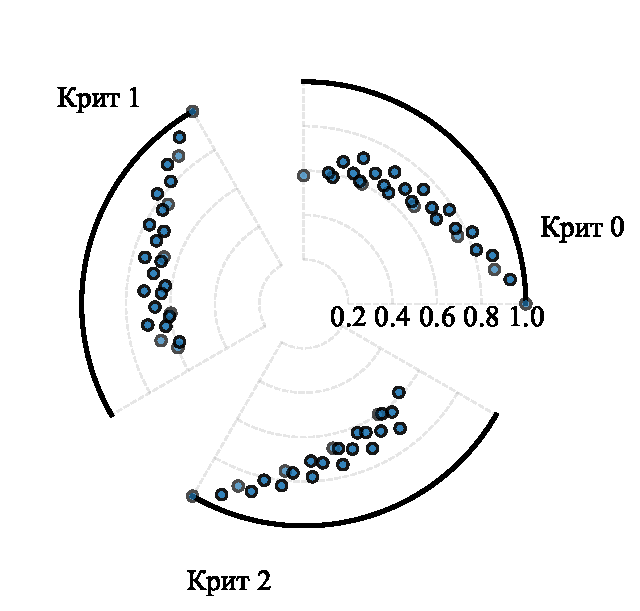
\includegraphics[]{part4/pareto_front_3_example_angular.pdf}
	}
	\caption{Пример визуализации фронта Парето для трех критериев с использованием angular mapping}
	\label{img4:pareto_front_angular_example}
\end{figure}

Для объективной оценки и сравнения полученных фронтов Парето применяется система формализованных метрик,
характеризующих различные аспекты распределения точек в пространстве критериев. Пусть имеется множество точек
фронта Парето $S = {\mathbf{x}^1, \mathbf{x}^2, \dots, \mathbf{x}^k}$, где каждый вектор $\mathbf{x}^i \in \mathbb{R}^m$ содержит значения целевых функций.

Основополагающей характеристикой является гиперобъем (hypervolume), определяемый выражением:
$$HV(S) = \mathrm{vol} \left(\bigcup_{\mathbf{x} \in S} [\mathbf{x}, \mathbf{r}]\right)$$
где $[\mathbf{x}, \mathbf{r}]$ -- ортогональный параллелепипед, ограниченный векторами $\mathbf{x}$ и референсной точкой $\mathbf{r}$, доминирующей все элементы множества $S$. 

Гиперобъем характеризует область пространства решений, охватываемую фронтом Парето, и является единственной метрикой, обладающей строгой монотонностью относительно отношения доминирования.
При необходимости сравнения двух фронтов Парето $F$ и $G$ применяется $\varepsilon$-индикатор:

$$\varepsilon(F, G) = \min { \varepsilon ,|, \forall \mathbf{g} \in G, \exists \mathbf{f} \in F : f_i \le \varepsilon g_i \text{ для всех } i }$$

Данный индикатор определяет минимальный коэффициент масштабирования, необходимый для доминирования одним множеством решений над другим.
Значение $\varepsilon$-индикатора менее единицы указывает на доминирование множеством $F$ множества $G$. Значение более единицы показывает необходимый коэффициент масштабирования множества $F$ для достижения доминирования.

Метрика покрытия $C(F,G)$ вычисляется как отношение количества доминируемых точек к общему числу точек:

$$C(F,G) = \frac{|{\mathbf{g} \in G \mid \exists \mathbf{f}\in F : \mathbf{f} \text{ доминирует } \mathbf{g} }|}{|G|}$$

При $C(F,G)$ близком к единице множество $F$ доминирует большинство точек множества $G$. При значениях близких к нулю доминирование практически отсутствует.

Для оценки равномерности распределения точек вдоль фронта применяется модифицированное расстояние Хаусдорфа:

$$D_H = \frac{1}{N-1}\sum_{i=1}^{N-1} \sqrt{\left(\frac{f_1^{(i+1)} - f_1^{(i)}}{s_1}\right)^2 + \left(\frac{f_2^{(i+1)} - f_2^{(i)}}{s_2}\right)^2}$$
где $f_1^{(i)}, f_2^{(i)}$ -- координаты i-й точки;
$s_1, s_2$ -- масштабирующие коэффициенты по соответствующим критериям, $N$ - количество точек фронта.

Коэффициент вариации расстояний между соседними точками определяется как:
$$CV = \frac{\sqrt{\frac{1}{N-1}\sum_{i=1}^{N-1}(d_i - \bar{d})^2}}{\bar{d}}$$
где $d_i$ -- евклидово расстояние между соседними точками, $\bar{d}$ - среднее расстояние между точками фронта.
Данный коэффициент характеризует степень неравномерности распределения точек.

Для оценки локальной плотности точек в трехмерном случае используется выражение:
$$\rho(f_1, f_2, f_3) = \frac{1}{N}\sum_{i=1}^N \frac{1}{V_i}$$
где $V_i$ -- объем тетраэдра, образованного текущей точкой и тремя ближайшими соседями. Высокие значения
плотности указывают на кластеризацию решений в определенных областях фронта.

Совокупное применение описанных метрик позволяет провести всесторонний анализ качества полученных решений и обеспечить объективное
сравнение эффективности различных алгоритмов управления. При этом каждая метрика характеризует определенный аспект распределения точек
в пространстве критериев, что дает возможность выявить как глобальные свойства фронта Парето, так и его локальные особенности.